\chapter{Lab network driver:网卡驱动实验}
\begin{introduction}
    \item 实现 Intel E1000 网卡的驱动
    \item 编写驱动程序的一般步骤
\end{introduction}

驱动程序是操作系统的重要组成部分,负责沟通操作系统和实际工作的硬件。在本次实验中,我们会在 xv6 中为一个现实中广泛使用的硬件: Intel E1000 网卡,编写驱动程序,从而体会编写驱动程序的一般步骤。

\section{实现 Intel E1000 网卡的驱动}

Intel E1000 网卡是一类常见的千兆以太网卡,广泛用于各类个人电脑和服务器中。由于其支持较为完善,且文档齐全,故而在我们的 qemu 中也有软件模拟的 E1000 设备,可供 xv6 实验使用。

在开始编写驱动程序前,我们需要获取 Intel 提供的关于 E1000 网卡的驱动的开发者文档 \textit{Intel E1000 Software Developer's Manual} \footnote{\url{https://pdos.csail.mit.edu/6.828/2021/readings/8254x_GBe_SDM.pdf}} ,其中包含了关于该网卡硬件特性和工作机制的说明。根据 xv6 的实验手册,我们主要需要关注以下内容:
\begin{enumerate}
    \item Section 2 :关于 E1000 的基本信息
    \item Section 3.2 :接收数据包的简介
    \item Section 3.3 和 Section 3.4 :发送数据包的简介
    \item Section 13 : E1000 使用到的寄存器
    \item Section 14 : E1000 的设备初始化过程
\end{enumerate}

大致浏览过上面的内容后,我们主要需要实现 \lstinline{kernel/e1000.c} 中的两个函数: 用于发送数据包的 \lstinline{e1000_transmit()} 和用于接收数据包的 \lstinline{e1000_recv()} 。用于初始化设备的 \lstinline{e1000_init()} 已经被实现好了,我们主要关注的是其涉及到的一些数据结构:
\begin{lstlisting}[language=C]
    #define TX_RING_SIZE 16
    static struct tx_desc tx_ring[TX_RING_SIZE] __attribute__((aligned(16)));
    static struct mbuf *tx_mbufs[TX_RING_SIZE];
    
    #define RX_RING_SIZE 16
    static struct rx_desc rx_ring[RX_RING_SIZE] __attribute__((aligned(16)));
    static struct mbuf *rx_mbufs[RX_RING_SIZE];
    
    // remember where the e1000's registers live.
    static volatile uint32 *regs;
    
    struct spinlock e1000_lock;
\end{lstlisting}

其中最重要的是两个环形缓冲区: \lstinline{tx_ring} 和 \lstinline{rx_ring} 。根据 \textit{Intel E1000 Software Developer's Manual} 上的描述,我们只需要将需要发送的数据包放入环形缓冲区中,设置好对应的参数并更新管理缓冲区的寄存器,即可视为完成了数据包的发送。此后网卡的硬件会自动在合适的时间将我们放入的数据包按照配置发送出去,在 \lstinline{kernel/e1000.c} 中的实现如下:
\begin{lstlisting}[language=C]
int
e1000_transmit(struct mbuf *m)
{
  //
  // Your code here.
  acquire(&e1000_lock);
  printf("e1000_transmit: called mbuf=%p\n",m);
  uint32 idx = regs[E1000_TDT]; 
  if (tx_ring[idx].status != E1000_TXD_STAT_DD)
  {
    __sync_synchronize();
    release(&e1000_lock);
    return -1;
  } else {
    if (tx_mbufs[idx] != 0)
    {
      mbuffree(tx_mbufs[idx]);
    }
    tx_ring[idx].addr = (uint64) m->head;
    tx_ring[idx].length = (uint16) m->len;
    tx_ring[idx].cso = 0;
    tx_ring[idx].css = 0;
    tx_ring[idx].cmd = 1;
    tx_mbufs[idx] = m;
    regs[E1000_TDT] = (regs[E1000_TDT] + 1) % TX_RING_SIZE;
  }
  release(&e1000_lock);
  return 0;
}
\end{lstlisting}

\begin{theorem}[关于锁和\lstinline{__sync_synchronize}]
    由于网卡本身就是仅有一份、只能独占的资源,故而对其进行操作时需要加锁。但在上面的代码中,当缓冲区满时,我们加入了一行 \lstinline{__sync_synchronize()} ,简单来说,其起到内存屏障的作用,即保证对内存的操作严格按照我们指定的顺序进行。若没有这个语句,则在发包缓冲区满时会出现一些难以调试的错误。
\end{theorem}

对于 \lstinline{e1000_recv()} 也依样画瓢,只是在将数据包拷贝出 \lstinline{rx_ring} 时,需要使用合适的函数。根据 xv6 实验手册的提示,我们无需自己实现该拷贝过程,而只需要调用 \lstinline{net.c} 中的 \lstinline{net_rx()} 即可。注意当网卡硬件产生一次中断后,我们的中断处理过程 \lstinline{e1000_intr} 会执行 \lstinline{regs[E1000_ICR] = 0xffffffff} 从而告知网卡我们已经完成了这次中断中所有数据包的处理,故而我们的 \lstinline{e1000_recv()} 需要将 \lstinline{rx_ring} 中的所有内容都拷贝出去,实现如下:
\begin{lstlisting}[language=C]
extern void net_rx(struct mbuf *);
static void
e1000_recv(void)
{
  //
  // Your code here.
  uint32 idx = (regs[E1000_RDT] + 1) % RX_RING_SIZE;
  struct rx_desc* dest = &rx_ring[idx];
  while (rx_ring[idx].status & E1000_RXD_STAT_DD)
  {
    acquire(&e1000_lock);

    struct mbuf *buf = rx_mbufs[idx];
    mbufput(buf, dest->length);
    if (!(rx_mbufs[idx] = mbufalloc(0)))
      panic("mbuf alloc failed");
    dest->addr = (uint64)rx_mbufs[idx]->head;
    dest->status = 0;
    regs[E1000_RDT] = idx;

    __sync_synchronize();
    release(&e1000_lock);
    net_rx(buf);
    idx = (regs[E1000_RDT] + 1) % RX_RING_SIZE;
    dest = &rx_ring[idx];
  }
}
\end{lstlisting}

这里同样需要加锁保证互斥,并使用 \lstinline{__sync_synchronize} 保证内存访问顺序,否则会使接收数据包的顺序产生变化。

至此,在 E1000 中我们需要做的工作便完成了。使用 \lstinline{make server} 运行 qemu 宿主机的服务器,然后用 \lstinline{make qemu} 编译并启动 xv6 ,在 xv6 中运行 \lstinline{nettests} ,可以得到如下图的结果:
\begin{figure}[H]
  \centering
  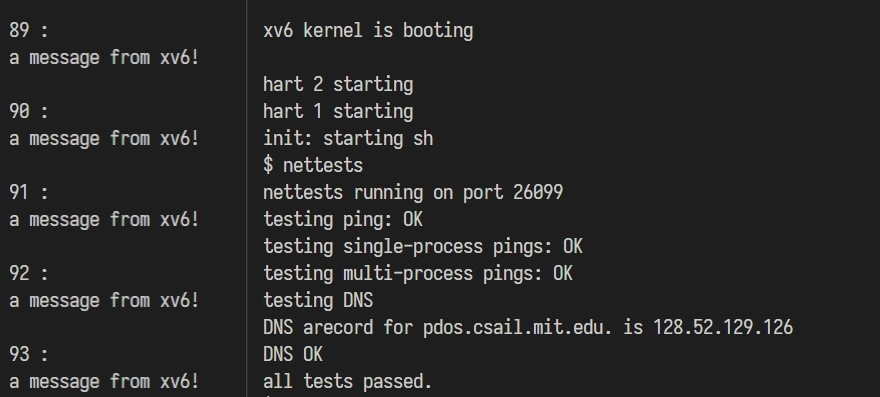
\includegraphics[width=0.8\textwidth]{net_nettests.jpg}
  \caption{网卡驱动的测试结果}
\end{figure}

可见结果符合预期。

\begin{proposition}[关于 DMA] 
    这里的 E1000 网卡驱动就是一个典型的使用 DMA ( Direct Memory Access ,直接存储器访问)的例子。网卡在初始化配置好后,会将收到的数据包和关于这些数据包的信息直接拷贝到内存的指定位置中,而无需 CPU 的参与。当网卡认为有必要让 CPU 处理这些数据时,就使用设备中断的方式通知 CPU 。从编写程序的角度看,我们并没有书写任何直接从网卡拷贝数据的代码,但对应的数据结构中已经被填充完成了;处理好一次中断收到的数据后,只要设置对应的寄存器,就可以告知网卡我们已经妥善处理其通过 DMA 传入的数据。
\end{proposition}

\paragraph*{实验结果} 在完成 Lab network driver 中的所有实验后,根据 MIT 6.S081 的传统,需要在实验目录下创建一个名为 \lstinline{time.txt} 文本文件,其中只包含一行,为完成该实验的小时数。先打开一个终端,在其中使用 \lstinline{make server} 运行 qemu 宿主机的服务器;然后打开另一个终端,在其中执行 \lstinline{make grade} ,即可对整个实验进行自动评分,笔者的结果如下:
\begin{figure}[H]
  \centering
  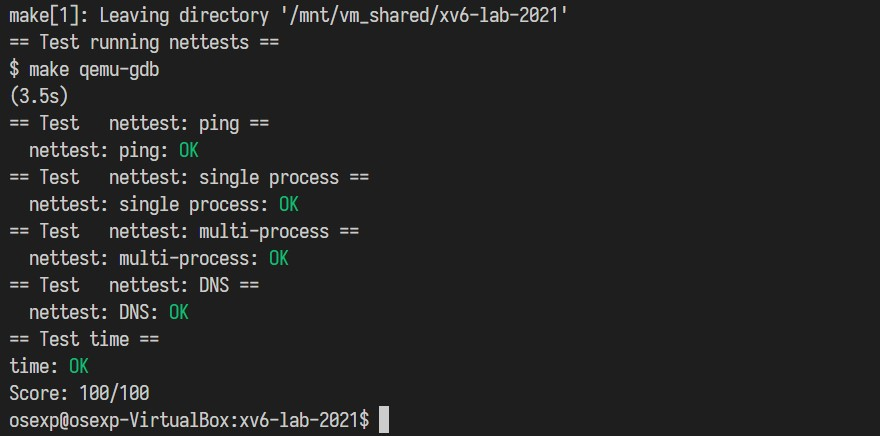
\includegraphics[width=0.8\textwidth]{net_grade.jpg}
  \caption{ Lab network driver 的测评结果}
\end{figure}
可见测试全部通过,得分为满分。

\section{小结:编写驱动程序的一般步骤}

由于现代大多数外设都通过 DMA 方式来与系统进行数据交换,故而很多外设驱动的编写的思路和本部分实验的一致。这里我们对编写驱动程序的一般步骤进行小结:
\begin{enumerate}
    \item 获取设备相关的文档
    \item 了解设备工作的大致过程
    \item 设计与设备交换数据的数据结构
    \item 创建对应的内核模块
    \item 编写设备初始化代码
    \item 编写具体功能
    \item 测试与验证
\end{enumerate}